\section{The Company}

\begin{quote}
    \color{dgreen} \textit{ATP was introduced by the Danish Parliament in 1964
    with the purpose of providing Danes with a state pension supplement. Today,
    ATP covers most of the Danish population who put money aside for their
    pension via ATP Livslang Pension.}

    \color{black}-- ATP 2020 annual report introduction
\end{quote}

\subsection{Overview}

Today, the ATP Group is Denmark’s largest pension company and Europe’s fourth
largest.\cite{top_pension} It is based in Hillerød and has around 3 000
employees, most of which currently work from home because of the pandemic. ATP
has since its creation expanded into a private financial processing and
investment enterprise which conducts billion-krone long term investments in
Danish companies through its 26 subsidiaries. The company recorded its second
best financial results ever in 2020, sustaining the Danish economy despite the
effects of COVID-19.\cite{about_atp}

In 1973, ATP began its processing business, which would eventually expand to a
variety of labour market schemes. From 1990, the Danish Parliament began a
series of amendments to the ATP Act which included improved benefits to ATP
members, and the addition of more groups not in the labour market to ATP
schemes. In 2011, the Parliament selected ATP as the manager of the welfare
state’s core benefits and it now handles state pensions, disability pensions,
rent subsidies, maternity/paternity benefits and family benefits. The company is
now Denmark’s largest provider and administrator of welfare and social security
schemes.\cite{atp_history}

\subsection{Structure \& Organisation}

\begin{figure}[H]
    \centering
        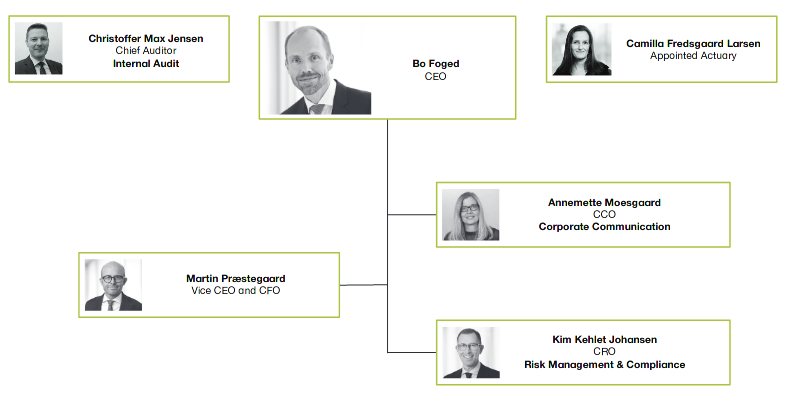
\includegraphics[width=\textwidth]{image2.png}
        \caption*{\textit{ATP's executive structure\cite{about_atp}}}
\end{figure}

The company is divided into two business areas: Pensions \& Investments and the
Processing Business. Both ultimately report to ATP’s Supervisory Board. There
exists a number of general departments similar to those present in most
companies: Legal, Communication \& External Relations, HR, Finance, IT, Sourcing
\& Contract Management and Risk Management \& Compliance. The Internal Audit and
Actuarial Department are completely separate from this structure and report
directly to the Supervisory Board.\cite{about_atp}

ATP Livslang Pension (Lifelong Pension) is simultaneously managed by a Board of
Representatives, the Supervisory Board and a CEO because of the critical nature
of this department as a mandatory and lifelong service for all Danish
citizens.\cite{about_atp,anno_report}

Within the Processing Business, there is a "Systems Architecture" team of seven
people into which I was admitted during my internship. To understand the purpose
of this activity, we must consider the entirety of the company's structure and
organisation. In essence, the stakeholders set the overall goals and
requirements to be implemented by the technically competent divisions. However,
in the realm of IT and communications, an intermediary step may be required to
translate and divide these goals into practical schemes which can be directly
implemented by developers, designers and others. In simpler terms, systems
architects determine and describe the requirements and course of action to be
taken in order to achieve an overall goal. They may also abstract and break down
the functions and interactions of a system into an "architecture", which allows
these systems to be assessed and optimised.\cite{sys_arch} Hence, this
profession is of crucial importance to a large and complex enterprise such as
ATP. These concepts will be further illustrated and detailed via my experience
in \hyperlink{subsection.2.1}{subsection 2.1}.

\subsection{Financial Overview}

\begin{figure}[H]
    \centering
        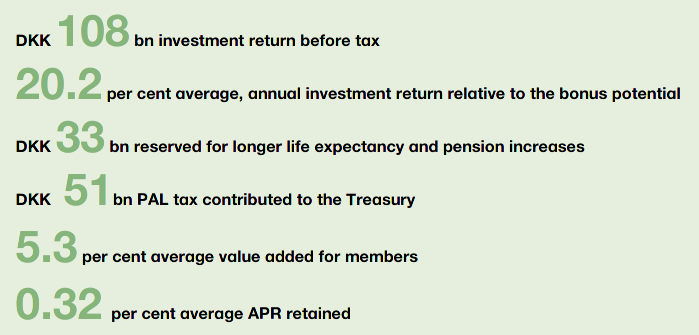
\includegraphics[width=\textwidth]{image5.png}
        \caption*{\textit{Financial summary of ATP's past 5
        years\cite{anno_report}}}
\end{figure}

Analysis of these statistics, especially the DKK 108 billion\footnote[0]{1€  =
DKK 7.44} return on investment before tax, shows that ATP has exhibited
considerable growth in these past five years. Furthermore, they report having
exceeded the Supervisory Board's expectations in 2020 for investment activities
with a result of DKK 17.6 billion.\cite{anno_report} During the COVID-19
pandemic, the Danish government triggered a number of measures to support the
economy. These measures include a recovery fund to invest in large Danish
companies threatened by the crisis and a one-time payment of DKK 1 000 to over
2.2 million residents. The ATP Group was selected to manage both of these
efforts, which renders apparent the close relationship between it and Danish
society, within which it primarily operates.\cite{covid_response} In the words
of CEO Bo Foged:

\begin{quote}
    \color{dgreen} \textit{ATP has been entrusted to solve important societal
    tasks for the benefit of all of Denmark}
\end{quote}
